\documentclass[12pt]{exam}

\newcommand{\course}{MTH 234 Summer 2021}
\newcommand{\qdate}{14.7 - Maximum and Minimum Values} %PUT DATE HERE
\newcommand{\quiz}{Group Work} 

    \usepackage[top=1in, bottom=1in, left=.45in, right=.45in]{geometry}
    \usepackage{amsmath,amsthm,amssymb,amstext}
    \usepackage{enumerate,enumitem}
    \usepackage{tikz,float,graphicx}
    \usepackage{microtype}
    \usepackage{bm,tikz}
        \usetikzlibrary{calc,positioning}
    \usepackage{multicol}
    \usepackage{nicematrix}
    \usepackage{cleveref}
    \usepackage[framemethod=tikz]{mdframed}
    \usepackage{graphicx}
    \usepackage[export]{adjustbox}
    
    %\newcommand{\course}{MTH 234 Summer 2021}
    %\newcommand{\qdate}{Equations of lines and planes} %PUT DATE HERE
    %\newcommand{\quiz}{Group Work} 
    
    \newcommand{\R}{\mathbb{R}}
    
    \newcommand{\ba}{\bm{a}}
    \newcommand{\bb}{\bm{b}}
    \newcommand{\bc}{\bm{c}}
    \newcommand{\bi}{\bm{i}}
    \newcommand{\bj}{\bm{j}}
    \newcommand{\bk}{\bm{k}}
    \newcommand{\br}{\bm{r}}
    \newcommand{\bv}{\bm{v}}
    \newcommand{\bu}{\bm{u}}
    \newcommand{\gen}[1]{\left\langle #1 \right\rangle}
    \newcommand{\pd}[2]{\dfrac{\partial #1}{\partial #2}}

\newtheorem*{theorem}{Theorem}
\surroundwithmdframed[]{theorem}

\theoremstyle{definition}
    \newtheorem*{definition}{Definition}
    \surroundwithmdframed[]{definition}
    \newtheorem*{info}{Useful Information}
    \surroundwithmdframed[]{info}
\theoremstyle{remark}
    \newtheorem*{remark}{Remark}
    \surroundwithmdframed[]{remark}
    

%%%%%%%%%%%%%%%%%%%%%%%
% HEADER AND FOOTER
%%%%%%%%%%%%%%%%%%%%%%%
\pagestyle{headandfoot}
\firstpageheadrule
\runningheadrule
\firstpageheader{\course}{\quiz}{\qdate}
\runningheader{\course}{\quiz}{\qdate}
\runningfooter{}{}{}


\usepackage{color}
\shadedsolutions
\definecolor{SolutionColor}{rgb}{0.8,0.9,1}

\usepackage{pgfplots}
    \pgfplotsset{every axis/.append style={
                    axis x line=middle,    % put the x axis in the middle
                    axis y line=middle,    % put the y axis in the middle
                    axis z line=middle,
                    axis line style={<->}, % arrows on the axis
                    xlabel={$x$},          % default put x on x-axis
                    ylabel={$y$},          % default put y on y-axis
                    zlabel={$z$},
                    grid=both,
                    %xtick={-4,...,-1,1,...,3},
                    %ytick={-1,1,}
    }}
    \pgfplotsset{compat=1.17}

\newcommand{\bif}{\quad\iff\quad}

\printanswers
%\noprintanswers

\begin{document}

\section*{\qdate}


\subsection*{Template}

\begin{questions}



%%%% what can you say 
\question Suppose \((1,1)\) is a critical point of a function \(f\) with continuous second derivatives. 
    What can you say about \(f\) and the point \((1,1)\) if 
    \begin{parts}
        \part 
            \[
                f_{xx}(1,1)=4,\qquad f_{x,y}=1,\qquad f_{y,y}=2
            \]
            \ifprintanswers
            \begin{solution}
                \[
                    D=f_{xx}f_{yy}-f_{xy}^2 = 4(2)-1^2=7>0
                \]
                Since \(f_{xx}(1,1)>0\) \(f(1,1)\) is a local minimum.
            \end{solution}
    \else
        \vfill
    \fi
        \part 
            \[
                f_{xx}(1,1)=4,\qquad f_{x,y}=3,\qquad f_{y,y}=21
            \]
            \ifprintanswers
        \begin{solution}
            Also a local minimum.
        \end{solution}
    \else
        \vfill
    \fi
    \end{parts}


%% find all crit points
\question Let \(f(x,y)=5xy(-3-x-y)\) 
\begin{parts}
    \part Show that the critical points of \(f(x,y)\) are 
    \[
        (0,0),(-3,0),(-1,-1),\quad \text{and} \quad (0,-3)
    \]
        \ifprintanswers
        \begin{solution}
            \begin{align*}
                f_x(x,y)&=5y(-3-x-y)-5xy=-5y(3+2x+y)=0\\
                f_y(x,y)&=5x(-3-x-y)-5xy=-5x(3+x+2y)=0
            \end{align*}
            So \(f_{x}(x,y)=0\) when \(y=0\) or \(3+2x+y=0\) and \(f_y(x,y)=0\) when \(x=0\) or \(3+x+2y=0\).

            If \(x=0\), then \(f_y=0\) and \(f_x=5y(3+y)\) so we get critical points when \(y=0\) or \(y=-3\). This gives \((0,0)\) and \((0,-3)\) as critical points.
            Similarly if \(y=0\) then \(f_x=0\) and \(f_y=5x(3+x)\) which (redundantly) gives us \((0,0)\) as a critical point but also \(-3,0\).

            If neither \(x\) or \(y\) are zero then \(x,y\) is a critical point if \(3+2x+y=0\Rightarrow y=-3-2x\) and \(3+x+2y=0\Rightarrow x=-3-2y\). 
            Solving gives \(x,y=-1\).
        \end{solution}
    \else
        \vfill
    \fi
    \part Find \(D(a,b)\) and \(f_{xx}(a,b)\) for each critical point \((a,b)\) above. 
        \ifprintanswers
        \begin{solution}
            \begin{align*}
                f_{xx} & = -10y\\
                f_{xy} & = -5(3+2x+y)-5y\\
                f_{yy} & = -10x
            \end{align*}
            \[
                \begin{NiceArray}{r r r r r}
                    ~ & f_{xx} & f_{yy} & f_{xy} & D(x,y)\\\hline
                (0,0)   & 0   & 0  & -15   & 0-(-15)^2 <0 \\
                (-3,0)  & 0   & 30 & 15 & 0(30)-(15)^2 < 0\\
                (0,-3) & 30 & 0 & 15 & 30(0)-15^2 <0\\
                (-1,-1) & 10 & 10 & 5 & (10)(10)-5^2 >0\\
                \end{NiceArray}
            \]
        \end{solution}
    \else
        \vfill
    \fi
    \part Classify each critical point of \(f\)
        \ifprintanswers
        \begin{solution}
            By the above \(f(x,y)\) has saddle points at \((0,0)\), \((-3,0)\) and \((0,-3)\) and a local minimum at \((-1,-1)\).
        \end{solution}
    \else
        \vfill
        \newpage
    \fi
\end{parts}

%%
\question Find and classify the four closest critical points of 
\[
    f(x,y)=3y\cos(-11x)
\] that are closes to the point \((0,0)\).
    \ifprintanswers
        \begin{solution}
            \begin{equation*}
                \begin{aligned}
                    f_{x}(x,y) & = 33y\sin(-11x)\\
                    f_{y}(x,y) &= 3\cos(-11x)
                \end{aligned} ~
                \begin{aligned}
                    f_{xx}(x,y) & = -363y\cos(-11x)\\
                    f_{xy}(x,y) & = 33\sin(-11x)\\
                    f_{yy}(x,y) & = 0
                \end{aligned}
            \end{equation*}
        From the above \(f_{x}(x,y)=0\) when \(y=0\) or \(-11x=\pi\cdot k\) for any integer \(k\). Similarly, \(f_y(x,y)=0\) when \(-11x=\pi/2+\pi\cdot k\), for any integer \(k\).

        The second statement is equivalent to 
        \[
            f_y(x,y)=0 \bif x= -\frac{\pi}{22}-\frac{\pi}{11}\cdot k = -\frac{\pi(1+2\cdot k)}{22}.
        \]
        Combining the above we have critical points at any value for \(k\), the closest to \((0,0)\) being when \(k=0,1,-1,2\),i.e. the points
        \[
            \left(-\frac{3\pi}{22},0\right), \left(-\frac{\pi}{22},0\right), \left(\frac{\pi}{22},0\right), \left(-\frac{3\pi}{22},0\right)
        \]
        \end{solution}
    \else
        \vfill
    \fi

\question Find all local minimimum and maximum values and saddle points for the function
\begin{parts}
    \part \(f(x,y)=x^2+xy+y^2+y\)
        \ifprintanswers 
        \begin{solution} 
            Minimum at \(f(1/3,-2/3)=-1/3.\)
        \end{solution}
    \else
        \vfill
    \fi
    \part \(f(x,y)=(x-y)(1-xy)\)
        \ifprintanswers
        \begin{solution}
            Saddle points at \((1,1)\)  and \((-1,-1)\).
        \end{solution}
    \else
        \vfill
        \newpage
    \fi
\end{parts}

\question Show that \(f(x,y)=x^2+4y^2-4xy+2\) has an infinite number of critical points and that \(D=0\) at each one. Then show that \(f\) has a local (and absolute) minimum at each critical point.
    \ifprintanswers
        \begin{solution}
            Note that \(f(x,y)=2+(x-2y)^2\)
            \begin{equation*}
                \begin{aligned}
                    f_x(x,y) &= 2x-4y\\
                    f_y(x,y) & = 8y-4x
                \end{aligned}\quad
                \begin{aligned}
                    f_{xx}(x,y) &=2\\                    
                    f_{yy}(x,y) &= 8
                \end{aligned}\quad 
                \begin{aligned}    
                    f_{xy}(x,y) &= -4\\
                        & 
                \end{aligned}
            \end{equation*}
            \(f(x,y)\) has a critical point when \(2x-4y=0\) and \((8y-4x=0)\), i.e. when
            \(x=2y\). So all points along the line \(x=2y\) are critical points. 

            For any such \((x,y)\)
            \[
                D(x,y)=2(8)-(-4)^2=0
            \]
            Note that since \(f(x,y)=2+(x-2y)^2\), we see \(f(x,y)\ge 2\). 
            If \(x=2y\) then \(f(x,y)=2+0=2\), so we see that at each critical point above the function has an absolute minimum.
        \end{solution}
    \else
        \vfill
    \fi

\question Find the absolute maximum and minimum values of
\[
    f(x,y)=x^2+y^2+x^2y+4\quad\text{over the region }\quad
    \{ (x,y) ~~|~~ |x| \le1,~|y|\le1\}r
\]
    \ifprintanswers
        \begin{solution}
            First we note 
            \begin{equation*}
                \begin{aligned}
                    f_{x}(x,y) & = 2x+2xy\\
                    f_{y}(x,y) & = 2y+x^2\\
                \end{aligned}~~
                \begin{aligned}
                    f_{xx}(x,y)&=2+2y\\
                    f_{yy}(x,y)&=2
                \end{aligned}~~
                \begin{aligned}
                    f_{xy}(x,y)&= 2x\\
                        &
                \end{aligned}~~
            \end{equation*}
            So critical points occur when \(f_{x}(x,y)=2x+2xy=2x(1+y)=0\) and
            \(f_{y}(x,y)=2y+x^2=0\). 
            This is the same as 
            \[
                x=0 \quad \text{and}\quad 2y+x^2=0
            \]
            or
            \[
                y=-1 \quad \text{and}\quad 2y+x^2=0
            \]
            If \(x=0\) then \(f_x(x,y)=0\) and \(f_y(x,y)=2y\). This gives the critical point \(0,0\). If \(y=-1\) then \(f_{x}(0,-1)=0\) and \(f_{y}(x,-1)=-2+x^2\). 

            Since we are in the rectangle \(-1\le x,y\le 1\), \(x=\pm\sqrt{2}\) is outside our domain and we do not get any additional critical points.

            So we have one critical point in the domain, \((0,0)\). 
            Since \(f_{xx}(0,0)=2\) and \(f_{xx}(0,0)f_{yy}(0,0)-f_{xy}(0,0)^2=4\), \(f(x,y)\) has a local (and possibly absolute) minimum \(f(0,0)=4\).

            We also need to check the boundary, which is described by the lines
            \[ 
                y=1,~y=-1,~x=-1,~\text{and}~x=1.
            \]
            \begin{center}
                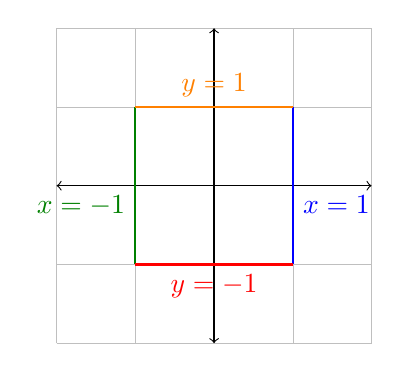
\begin{tikzpicture}
                    \draw[very thin,gray!50] (-2,-2) grid (2,2);
                    \draw[thin,<->] (-2,0)--(2,0);
                    \draw[thin,<->] (0,-2)--(0,2);
                    \draw[thick,blue] (1,1)--(1,-1) node[midway,anchor=north west] {$x=1$};
                    \draw[thick,green!50!black] (-1,1)--(-1,-1) node[midway,anchor=north east] {$x=-1$};
                    \draw[thick,red] (-1,-1)--(1,-1) node[midway,anchor=north] {$y=-1$};
                    \draw[thick,orange] (-1,1)--(1,1) node[midway,anchor=south] {$y=1$};
                \end{tikzpicture}
            \end{center}

            \noindent \(\bm{y=1}\)\\
            When \(y=1\), \(f(x,1)=2x^2+5,~~-1\le x\le 1\). The critical points along this line for \(f(x,1)\) are given by \(f'(x,1)=4x=0\), i.e at the point \(0,1\).
            Then the potential mins and maxes along this edge are given by 
            \[
                f(-1,1)=7=f(1,1)\quad \text{and}\quad f(0,1)=5.
            \]

            \noindent \(\bm{y=-1}\)\\
            When \(y=-1\), \(f(x,-1)=5\).


            \noindent \(\bm{x=1}\)\\
            When \(x=-1\), \(f(-1,y)=y^2+y+5\).
            Since \(f'(-1,y)=2y+1\), we have a critical point at \(-1,-1/2\). Checking this and the endpoints of this part of the boundary, we have
            \[
                f(1,-1/2)=\frac{19}{4},\quad f(1,-1)=5,\quad \text{and}~ f(1,1)=7.
            \]

            \noindent \(\bm{x=-1}\)\\
            When \(x=-1\), a similar process as above gives 
            \[
                f(-1,-1/2)=\frac{19}{4},\quad f(-1,-1)=5,\quad \text{and}~ f(-1,1)=7.
            \]
            
            It follows that over the region above, \(f(x,y)\) has absolute minimum \(f(0,0)=4\) and absolute maximum \(f(1,1)=f(-1,1)=7\).

            
        \end{solution}
    \else
        \vfill
    \fi

\question Find the absolute maximum and minimum values of 
\[
    f(x,y)=x^2+y^2-2x \quad \text{over the closed triangular region with vertices} \quad (2,0),(0,2),(0,-2).
\]
    \ifprintanswers
        \begin{solution}
            The domain is 
            \begin{center}
                \begin{tikzpicture}
                    \foreach \x/\y in {2/0,0/2,0/-2}
                    {
                        \draw[fill=black] (\x,\y) circle[radius=1pt];
                        \node[right] at (2,0) {$(2,0)$};
                        \node[above] at (0,2) {$(0,2)$};
                        \node[below] at (0,-2) {$(0,-2)$};
                    }
                    \draw (2,0)--(0,2)--(0,-2)--(2,0);
                \end{tikzpicture}
            \end{center}
            bounded by 
            \begin{align*}
                x&=0,~~ -2\le y\le y\\
                y&=2-x,~~ 0\le x\le 2\\
                y&=x-2,~~ 0\le x\le 2
            \end{align*}//

            \begin{equation*}
                \begin{aligned}
                    f_x(x,y)&=2x-2\\
                    f_y(x,y)&=2y
                \end{aligned}~~~~
                \begin{aligned}
                    f_{xx}(x,y)&=2
                    f_{yy}(x,y)&=2
                    f_{xy}(x,y)&=0
                \end{aligned}
            \end{equation*}
            The only critical point occurs when \(2x-2=0=2y\), at the point \((1,0)\).

            Since \(f_{xx}f_{yy}-f_{xy}^2=4\) and \(f_{xx}(1,0)=2\), \(f(x,y)\) has a local minimum of \(f(1,0)=2\).

            \noindent \(\bm{x=0}\)
            Along this line \(f(0,y)=y^2\) with \(-2\le y\le2\). A critical point for \(f(0,y)\) occurs at \((0,0)\). 
            Including the end points we will check the points \((0,0),(0,-2),(0,2)\).

            \noindent \(\bm{y=2-x}\)
            \(f(x,2-x)= \)


            \begin{equation*}
                \begin{aligned}
                    f(0,0)&=0\\
                    f(0,-2)&=4\\
                    f(0,2)&=4
                \end{aligned}
            \end{equation*}
        \end{solution}
    \else
        \vfill
        \newpage
    \fi

\question Find the shortest distance from the point \((2,0,-3)\) to the plane \(x+y+z=1\).
    \ifprintanswers
        \begin{solution}
            The distance from a point \((x,y,z)\) to \((2,0,-3)\) is given by 
            \[
                d=\sqrt{(x-2)^2+y^2+(z+3)^2}.
            \]
            Our goal is to minimize this distance with the restriction that \(x+y+z=1\). A trick to make this easier is to instead minimize \(d^2=(x-2)^2+y^2+(z+3)^2\). Using the equation \(z=1-x-y\) this amounts to finding the values of \(x\)  and \(y\) that minimize
            \[
                f(x,y)=(x-2)^2+y^2+(4-x-y)^2.
            \]

            From 
            \begin{equation*}
                \begin{aligned}
                    f_x(x,y)&=2(x-2)+2(4-x-y)(-1)=4x+2y-12\\
                    f_y(x,y)&=2x+4y-8
                \end{aligned}~~
                \begin{aligned}
                    f_{xx}(x,y)&=4
                    f_{yy}(x,y)&=4
                \end{aligned}~~
                \begin{aligned}
                    f_{xy}(x,y)&=2
                        &
                \end{aligned}~~
            \end{equation*}
            The function has critical points when 
            \[
                4x+2y-12=0\Rightarrow y=6-2x
            \]
            and
            \[
                2x+4y-8=0\Rightarrow y=2-\frac{1}{2}x.
            \]
            If these equations are both true, then 
            \[
                6-2x=2-\frac{1}{2}x \bif 4=\frac{3}{2}x \bif x=\frac{8}{3}
            \]
            which means \(y=6-2(8/3)=2/3\) and \(z=1-\frac{8}{3}-\frac{2}{3}=-7/3\),
            and the closest point on the plane is 
            \[
                \left(\frac{8}{3},\frac{2}{3},-\frac{7}{3}\right) 
            \]
            which is a distance of
            \[
                \sqrt{
                    \left(\frac{8}{3}-2 \right)^2
                    +\left(\frac{2}{3}\right)^2+\left(-\frac{7}{3}+3\right)^2
                }=2/\sqrt{3}.
            \]

        \end{solution}
    \else
        \vfill
    \fi

\question A rectangle with length 4 and width 6 is cut into four smaller rectangles by two lines parallel to the sides. Find the maximum and minimum values of the sum of the squares of the areas of the smaller rectangles.
    \ifprintanswers
        \begin{solution}~

            The image below represents the situation described above. 
            \begin{center}
            \begin{tikzpicture}
                \node at (0,0) (a) {};
                \node at (0,-6) (b) {};
                \node at (4,-6) (c) {};
                \node at (4,0) (d) {};
                \node at (0,-3) (ab) {};
                \node at (2,-6) (bc) {};
                \node at (4,-3) (cd) {};
                \node at (2,0) (da) {};
                \draw (a.center) -- (b.center) -- (c.center) -- (d.center) -- (a.center);

                \draw [decorate,decoration={brace,amplitude=10pt}] ($(a)+(0,0.25)$) -- ($(d)+(0,0.25)$) node[midway,above,yshift=1em] {$4$};
                \draw [decorate,decoration={brace,amplitude=10pt,mirror}] ($(a)+(-.25,0)$) -- ($(b)+(-.25,0)$) node[midway,left,xshift=-1em] {$6$};
                
                \draw [decorate,decoration={brace,amplitude=6pt,mirror}] ($(b)+(0,-.25)$) -- ($(1.5,-6)+(0,-.25)$) node[midway,below,yshift=-1em] {$x$};
                \draw [decorate,decoration={brace,amplitude=6pt,mirror}] ($(1.5,-6)+(0,-.25)$) -- ($(c)+(0,-.25)$)  node[midway,below,yshift=-1em] {$4-x$};

                \draw [decorate,decoration={brace,amplitude=6pt,mirror}] ($(c)+(.25,0)$) -- ($(4,-3.5)+(0.25,0)$) node[midway,right,xshift=1em] {$y$};
                \draw [decorate,decoration={brace,amplitude=6pt,mirror}] ($(4,-3.5)+(0.25,0)$) -- ($(d)+(.25,0)$)  node[midway,right,xshift=1em] {$6-y$};            

                \draw[dashed] (1.5,0)--(1.5,-6);
                \draw[dashed] (0,-3.5)--(4,-3.5);
            \end{tikzpicture}
            \end{center}

            The smaller rectangles, starting with the upper left and moving counter-clockwise, have areas 
            \[
                x(6-y),xy,(4-x)y,\quad \text{and}~~(4-x)(6-y)
            \] respectively.

            Summing the squares of these values gives
            \begin{align*}
                a(x,y) & = x^2(6-y)^2+x^2y^2+(4-x)^2y^2+(4-x)^2(6-y)^2 = 4(x^2-4x+8)(y^2-6y+18),\quad 0\le x\le 4, 0 \le y\le 6.\\
            \end{align*}
            \begin{equation*}
                \begin{aligned}
                    a_x(x,y) &= 4(2x-4)(y^2-6y+18)\\
                    a_y(x,y) & = 4(x^2-4x+8)(2y-6)
                \end{aligned}~~
                \begin{aligned}
                    a_{xx}(x,y) &= 8(y^2-6y+18)\\
                    a_{yy}(x,y) & = 8(x^2-4x+8)
                \end{aligned}~~
                \begin{aligned}
                    a_{xy}(x,y) &= 4(2x-4)(2y-6)\\
                    &
                \end{aligned}~~
                \end{equation*}

                Notice that \(y^2-6y+18=0\) and \(x^2-4x+8=0\) have no real solutions. Then 
                \[
                    a_x(x,y)=0 \bif x=2 \quad\text{and}\quad a_y(x,y)=0 \bif y=3
                \]
                Which gives the critical point \((2,3)\) with \(a(2,3)=144\).

                The boundary of the domain of this function is given by the lines \(x=0,x=4,y=0,y=6\).

                \noindent \(\bm{x=0}\)\\
                \[
                    a(0,y) = 32(y^2-6y+18),\quad a'(0,y)=32(2y-6) 
                \] so we will check points \((0,0)\), \(0,3\), and \((0,6)\).

                \noindent \(\bm{x=4}\)\\
                \[
                    a(4,y) = 32(y^2-6y+18),\quad a'(4,y)=32(2y-6)
                \] 
                so we check \((4,0)\),\((4,3)\),(4,6).

                Similarly, setting \(y=0\) and \(y=6\) gives us points
                \[
                    (0,0), (2,0), (4,0)\quad \text{and}\quad (0,6), (2,6), (4,6)
                \]
                respectively. 

                The maximum possible value is given when 
                \[
                    a(0,0)=a(4,0)=a(4,6)=a(0,6)=576
                \] and the minimum value is given by 
                \[
                    a(2,3)=144.
                \]

        \end{solution}
    \else
        \vfill
    \fi 

\end{questions}

\end{document}

%soln : Question environment
    \ifprintanswers
        \begin{solution}
        \end{solution}
    \else
        \vfill
    \fi